\documentclass[tikz,border=1mm]{standalone}
\usetikzlibrary{shapes.geometric, arrows.meta}

\begin{document}
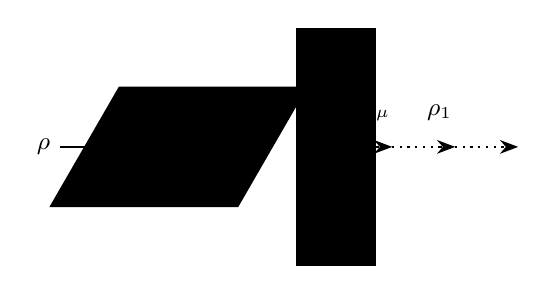
\begin{tikzpicture}[thick,
    amplifier/.style={fill=black, draw, trapezium, trapezium left angle=60, trapezium right angle=-60, minimum width=1cm, minimum height=1.5cm},
    beamsplitter/.style={fill=black, draw, rectangle, minimum width=1cm, minimum height=3cm},
    arrow/.style={->, >=Stealth, dotted, thick},
    label/.style={black, font=\small}
]

% Amplifier
\node[amplifier] (amp) at (0,0) {};
\node[label] at (amp.center) {Amp};

% Beam Splitter
\node[beamsplitter] (bs) at (2,0) {};
\node[label] at (bs.center) {B.S.};

% Input arrow
\draw[-Latex, thick] (-1.5,0) -- (-0.5,0);
\node[label, left] at (-1.5,0) {$\rho$};

% Output arrows
\foreach \i/\j in {0.8/\rho_1, 0/\rho_\mu, -0.8/\rho_N} {
    \draw[arrow] (bs.east) ++(\i,0) -- ++(1,0);
    \node[label, above] at (bs.east) [xshift=\i cm, yshift=0.2cm] {$\j$};
}

\end{tikzpicture}
\end{document}